% !TEX program = xelatex
\documentclass[aspectratio=169,11pt]{beamer}
\makeatletter
\def\input@path{{../theme/}}
\makeatother

\usepackage{ctex,hyperref}
\usepackage[T1]{fontenc}
\usepackage{amsmath,booktabs,tabularx,graphicx,tikz,colortbl}
\usepackage{RenminUniv}
\usetikzlibrary{positioning,arrows.meta,calc,fit,decorations.pathreplacing}

% Keep the copied visual system readable without letting dense frames spill
% into the footer.
\linespread{1.0}

\graphicspath{{../theme/pic/}{../assets/}}

\definecolor{navyBlue}{HTML}{3A4046}
\definecolor{navyDeep}{HTML}{2F3439}
\definecolor{accentRed}{HTML}{9E2A2B}
\definecolor{softBlue}{HTML}{F5F6F5}
\definecolor{softGray}{HTML}{FAFAF9}
\definecolor{deepGray}{HTML}{2F3439}
\definecolor{mutedGray}{HTML}{6D747B}
\definecolor{lineGray}{HTML}{D4D9DD}
\definecolor{softRed}{HTML}{F9EEEE}
\definecolor{paperWhite}{HTML}{FEFEFD}
\definecolor{gateGreen}{HTML}{E6F4EA}
\definecolor{gateGreenLine}{HTML}{2E7D5B}

\setbeamertemplate{navigation symbols}{}
\setbeamertemplate{background}{%
    \begin{tikzpicture}[remember picture,overlay]
        \ifnum\insertframenumber=1
            \node[anchor=south west,inner sep=0,opacity=0.40] at (current page.south west)
                {
\includegraphics[width=\paperwidth,height=\paperheight]{../theme/pic/background.pdf}};
        \else
            \node[anchor=south west,inner sep=0,opacity=0.13] at (current page.south west)
                {
\includegraphics[width=\paperwidth,height=\paperheight]{../theme/pic/background.pdf}};
        \fi
    \end{tikzpicture}%
}
\setbeamerfont{frametitle}{size=\large,series=\bfseries}
\setbeamerfont{block title}{size=\normalsize,series=\bfseries}
\setbeamercolor{normal text}{fg=deepGray}
\setbeamercolor{background canvas}{bg=paperWhite}
\setbeamercolor{frametitle}{bg=paperWhite,fg=accentRed}
\setbeamercolor{block title}{bg=navyBlue,fg=white}
\setbeamercolor{block body}{bg=softBlue,fg=deepGray}
\setbeamercolor{title}{bg=paperWhite,fg=accentRed}
\setbeamercolor{titlelike}{bg=paperWhite,fg=accentRed}
\setbeamercolor{author in head/foot}{bg=paperWhite,fg=mutedGray}
\setbeamercolor{institute in head/foot}{bg=paperWhite,fg=mutedGray}
\setbeamercolor{title in head/foot}{bg=paperWhite,fg=mutedGray}
\setbeamercolor{frame number}{fg=accentRed}
\setbeamercolor{upper separation line foot}{bg=accentRed}
\setbeamercolor{lower separation line foot}{bg=lineGray}
\setbeamercolor{palette primary}{bg=paperWhite,fg=accentRed}
\setbeamercolor{palette secondary}{bg=softGray,fg=mutedGray}
\setbeamercolor{palette tertiary}{bg=softGray,fg=mutedGray}
\setbeamercolor{palette quaternary}{bg=softGray,fg=mutedGray}
\setbeamercolor{structure}{fg=accentRed}
\setbeamersize{text margin left=0.55cm,text margin right=0.55cm}
\setlength{\tabcolsep}{0.13cm}
\renewcommand{\arraystretch}{1.16}

\newcommand{\key}[1]{\textcolor{accentRed}{\textbf{#1}}}
\newcommand{\muted}[1]{\textcolor{mutedGray}{#1}}
\newcommand{\smallnote}[1]{{\scriptsize\textcolor{mutedGray}{#1}}}
\newcommand{\keynote}[1]{{\footnotesize\textcolor{navyBlue}{#1}}}
\newcommand{\sectionhead}[1]{%
    {\textcolor{navyBlue}{\bfseries\normalsize #1}}\\
    {\textcolor{accentRed}{\rule{\linewidth}{0.65pt}}}\\
}
\newcommand{\cellhead}[1]{\textcolor{accentRed}{\bfseries\normalsize #1}}
\newcommand{\code}[1]{\texttt{\small #1}}
\newcommand{\takeaway}[1]{%
    \fcolorbox{accentRed}{softRed}{\parbox{0.78\textwidth}{\centering\color{accentRed}\Large\bfseries #1}}}
\newcommand{\compacttakeaway}[1]{%
    \fcolorbox{accentRed}{softRed}{\parbox{0.78\textwidth}{\centering\color{accentRed}\normalsize\bfseries #1}}}
\newcommand{\stagecard}[5]{%
    \node[#1,text width=4.00cm,minimum width=4.50cm,minimum height=3.15cm,align=center] at (#2,-0.15) {%
        \begin{minipage}[t][2.75cm][t]{4.00cm}
            \centering
            {\textcolor{accentRed}{\Large\bfseries #3}}\\[1mm]
            {\textcolor{navyBlue}{\bfseries #4}}\\[1.5mm]
            #5
        \end{minipage}%
    };
}

\tikzset{
    card/.style={draw=lineGray,fill=paperWhite,rounded corners=4pt,
        inner sep=6pt,align=center,font=\small},
    accentcard/.style={draw=accentRed!70,fill=softRed,rounded corners=4pt,
        inner sep=6pt,align=center,font=\small},
    gatebox/.style={draw=gateGreenLine,fill=gateGreen,rounded corners=4pt,
        inner sep=6pt,align=center,font=\small},
    tensor/.style={draw=mutedGray!65,fill=white,rounded corners=2pt,
        minimum width=1.0cm,minimum height=0.62cm,align=center,font=\scriptsize},
    flow/.style={draw=lineGray,fill=paperWhite,rounded corners=3pt,
        minimum width=2.45cm,minimum height=0.72cm,align=center,font=\small},
    flowgreen/.style={draw=gateGreenLine!75,fill=gateGreen,rounded corners=3pt,
        minimum width=2.45cm,minimum height=0.72cm,align=center,font=\small},
    arrow/.style={->,draw=mutedGray!85,line width=0.85pt},
    dottedarrow/.style={->,dashed,draw=accentRed,line width=0.7pt},
    thinbox/.style={draw=lineGray,rounded corners=3pt,align=center,
        inner sep=5pt,font=\small}
}


\author{DefaultGroup｜中国人民大学 CCIR 参赛队}
\title{基于 Agent 轨迹的检索器训练}
\institute{中国人民大学高瓴人工智能学院}
\date{}

\begin{document}
\begingroup
    \setbeamertemplate{footline}{}
    \begin{frame}
        \begin{center}
            \vspace*{0.55cm}
            {\color{accentRed}\LARGE\bfseries\inserttitle\par}
            \vspace{0.45cm}
            {\color{navyBlue}\large 官方 LRAT Training pairs 的训练与验证\par}
            \vspace{1.15cm}
            {\color{navyBlue}\large\insertauthor\par}
            \vspace{0.32cm}
            {\color{mutedGray}\normalsize\insertinstitute\par}
            \vfill
            
\includegraphics[width=0.22\linewidth]{Renmin_Univ_Logo.eps}
            \vspace*{0.55cm}
        \end{center}
    \end{frame}
\endgroup

\begin{frame}{团队与分工}
    \begin{center}
        \keynote{我们分别负责数据核验、数据切分、模型训练、榜单评测和复现交付。}
    \end{center}
    \begin{center}
        \begin{tikzpicture}[node distance=0.36cm and 0.36cm]
            \node[card,text width=5.20cm,minimum height=3.18cm] (a) {
                \textcolor{accentRed}{\Large\bfseries 01}\quad 刘琦（队长）\\[1.5mm]
                \textcolor{navyBlue}{\bfseries 13798122637}\\[1.5mm]
                \scriptsize 技术分工：整体方案设计与答辩协作；\\[0.5mm]
                };
            \node[card,text width=5.20cm,minimum height=3.18cm] (b) [right=of a] {
                \textcolor{accentRed}{\Large\bfseries 02}\quad 赵梓名\\[1.5mm]
                \textcolor{navyBlue}{\bfseries 18875820386}\\[1.5mm]
                \scriptsize 技术分工：训练、评测与交付协作；\\[0.5mm]};
        \end{tikzpicture}
    \end{center}
    \begin{center}
        \begin{tikzpicture}
            \node[accentcard,text width=11.55cm,minimum height=0.84cm] {
                \textbf{队伍信息}\quad Team ID：362259\quad Record ID：998912\\};
        \end{tikzpicture}
    \end{center}
\end{frame}

\begin{frame}{1. 研究背景：检索器的服务对象从人转向 Agent}
    \begin{center}
        \keynote{当检索器的服务对象从人转向 Agent，检索结果的消费方式与训练监督来源也随之变化\textsuperscript{[1]}。}
    \end{center}

    \vspace{0.5mm}
    \begin{center}
        \begin{tikzpicture}
            \node[font=\small\bfseries,text=navyBlue] at (-1.10,1.42) {Human Search};
            \node[font=\small\bfseries,text=navyBlue] at (5.20,1.42) {训练数据};

            \node[flow,minimum width=2.85cm,minimum height=0.72cm,font=\small] (hq) at (-4.30,0.62)
                {用户 query};
            \node[flowgreen,minimum width=2.85cm,minimum height=0.72cm,font=\small] (hr) at (-1.10,0.62)
                {排序结果};
            \node[flow,minimum width=2.85cm,minimum height=0.72cm,font=\small] (hf) at (2.10,0.62)
                {click / dwell};
            \draw[arrow] (hq) -- (hr);
            \draw[arrow] (hr) -- (hf);

            \node[card,minimum width=2.00cm,minimum height=0.72cm,font=\scriptsize] (hlog) at (5.35,0.62)
                {Human Log};

            \draw[->,line width=1.0pt,accentRed] (-1.10,0.22) -- (-1.10,-0.62);
            \node[font=\scriptsize\bfseries,text=accentRed,align=right,anchor=east]
                at (-1.34,-0.18) {检索结果不再是终点};
            \node[font=\scriptsize\bfseries,text=accentRed,align=left,anchor=west]
                at (-0.86,-0.18) {而是 Agent 后续推理的输入};

            \draw[->,line width=1.0pt,accentRed] (5.35,0.22) -- (5.35,-1.36);

            \node[font=\small\bfseries,text=navyBlue] at (-1.10,-0.88) {Agentic Search};
            \node[accentcard,minimum width=2.00cm,minimum height=0.72cm,font=\scriptsize] (atraj) at (5.35,-1.73)
                {Agent Trajectory};

            \node[flow,minimum width=2.30cm,minimum height=0.72cm,font=\scriptsize] (aq) at (-5.00,-1.73)
                {中间 query};
            \node[flowgreen,minimum width=2.30cm,minimum height=0.72cm,font=\scriptsize] (as) at (-2.45,-1.73)
                {snippet};
            \node[flow,minimum width=2.30cm,minimum height=0.72cm,font=\scriptsize] (ab) at (0.10,-1.73)
                {Browse};
            \node[flowgreen,minimum width=2.30cm,minimum height=0.72cm,font=\scriptsize] (ar) at (2.65,-1.73)
                {后续 reasoning};
            \draw[arrow] (aq) -- (as);
            \draw[arrow] (as) -- (ab);
            \draw[arrow] (ab) -- (ar);
        \end{tikzpicture}
    \end{center}

    \vspace{-1mm}
    {\centering\tiny\textcolor{mutedGray}{[1] Yuqi Zhou et al., \textit{Learning to Retrieve from Agent Trajectories}, SIGIR 2026.}\par}
    \vspace{-1mm}
    \begin{center}
        \compacttakeaway{如何利用 Agent Trajectory 训练面向 Agentic Search 的 retriever？}
    \end{center}
\end{frame}

\begin{frame}{2. 从 LRAT 论文到本次训练：三个具体问题}
    \begin{center}
        \keynote{赛题提供 Training pairs、Agent trajectories 和 Corpus，并指定 Qwen3-Embedding-0.6B 作为基础模型。\\ 在不重新生成 trajectory 的前提下，如何可靠地利用已有 Training pairs 完成训练？}
    \end{center}

    \begin{center}
        \begin{tikzpicture}[node distance=0.14cm and 0.14cm]
            \node[card,text width=4.46cm,align=left] (signal) {
                \begin{minipage}[t][2.00cm][t]{4.46cm}
                    \centering\textcolor{accentRed}{\Large\bfseries 01}\\[-0.5mm]
                    \textcolor{navyBlue}{\bfseries 每条 pair 能否回到轨迹？}\\[1.0mm]
                    \scriptsize
                    核对 query、正例、负例和样本权重与 Search / Browse / reasoning 的映射，并确认文档均在 Corpus 中。
                \end{minipage}};
            \node[card,text width=4.46cm,align=left] (leak) [right=of signal] {
                \begin{minipage}[t][2.00cm][t]{4.46cm}
                    \centering\textcolor{accentRed}{\Large\bfseries 02}\\[-0.5mm]
                    \textcolor{navyBlue}{\bfseries 相同 query 如何避免跨集合？}\\[1.0mm]
                    \scriptsize
                    同一 normalized query 可能对应多条 source rows，随机切分会让相同 query 同时出现在 train 和 dev。
                \end{minipage}};
            \node[accentcard,text width=4.46cm,align=left] (cost) [right=of leak] {
                \begin{minipage}[t][2.00cm][t]{4.46cm}
                    \centering\textcolor{accentRed}{\Large\bfseries 03}\\[-0.5mm]
                    \textcolor{navyBlue}{\bfseries 训练轮数和学习率怎样选择？}\\[1.0mm]
                    \scriptsize
                    完整训练成本较高，因此先固定样本组装和损失，再分别用 A 榜和 dev1500 选择 epoch 与 LR。
                \end{minipage}};
        \end{tikzpicture}
    \end{center}

    \vspace{-3mm}
    \begin{center}
        \textcolor{navyBlue}{\bfseries 针对这三个问题，我们最终采用四个步骤：}
    \end{center}
    \begin{center}
        \begin{tikzpicture}[node distance=0.30cm and 0.30cm]
            \node[flowgreen,minimum width=2.50cm,minimum height=1.10cm,font=\scriptsize,align=center,inner sep=1.0pt] (a) {Training pair\\追溯核验};
            \node[flow,minimum width=2.50cm,minimum height=1.10cm,font=\scriptsize,align=center,inner sep=1.0pt] (b) [right=of a] {Normalized query\\整组切分};
            \node[flowgreen,minimum width=2.50cm,minimum height=1.10cm,font=\scriptsize,align=center,inner sep=1.0pt] (c) [right=of b] {固定候选\\加权训练};
            \node[flow,minimum width=2.50cm,minimum height=1.10cm,font=\scriptsize,align=center,inner sep=1.0pt] (d) [right=of c] {受控实验\\确定 epoch 与 LR};
            \draw[->,draw=mutedGray!95,line width=1.20pt,>=Latex] (a) -- (b);
            \draw[->,draw=mutedGray!95,line width=1.20pt,>=Latex] (b) -- (c);
            \draw[->,draw=mutedGray!95,line width=1.20pt,>=Latex] (c) -- (d);
        \end{tikzpicture}
    \end{center}
\end{frame}

\begin{frame}{3.1 LRAT 训练信号与来源核验}
    \begin{center}
        \keynote{LRAT 用 Browse 区分候选正负：已 Browse 文档作候选正例，未 Browse 候选入负例池。}
    \end{center}

    \centering
    \begin{tikzpicture}[node distance=0.25cm and 0.62cm]
        \node[font=\footnotesize\bfseries,text=navyBlue,anchor=center] at (0,1.15)
            {LRAT 论文中的训练信号形成};

        \node[flow,minimum width=2.30cm,minimum height=0.64cm,
            text width=2.18cm,font=\scriptsize,align=center,inner sep=2pt] (search) at (-5.15,0.48)
            {Search(query)\\[-0.2mm]top-K candidates};
        \node[flowgreen,minimum width=2.10cm,minimum height=0.64cm,
            text width=1.98cm,font=\scriptsize,align=center,inner sep=2pt] (browse) at (-1.98,0.48)
            {Browse(doc)\\[-0.2mm]先作候选正例};
        \node[flow,minimum width=3.05cm,minimum height=0.64cm,
            text width=2.93cm,font=\scriptsize,align=center,inner sep=2pt] (reason) at (1.28,0.48)
            {post-Browse reasoning\\[-0.2mm]再过滤无效信号};
        \node[accentcard,minimum width=2.65cm,minimum height=0.62cm,
            text width=2.53cm,font=\scriptsize,align=center,
            inner xsep=2pt,inner ysep=1.5pt] (pair) at (4.965,0.48)
            {Training pair\\[-0.2mm]query / pos / neg};

        \draw[arrow] (search.east) -- (browse.west);
        \draw[arrow] (browse.east) -- (reason.west);
        \draw[arrow] (reason.east) -- (pair.west);

        \node[flowgreen,minimum width=2.45cm,minimum height=0.62cm,
            text width=2.55cm,font=\scriptsize,align=center] (audit_pair) at (-4.90,-1.10)
            {Training pair};
        \node[flow,minimum width=4.00cm,minimum height=0.62cm,
            text width=3.90cm,font=\scriptsize,align=center] (events) at (-0.35,-1.10)
            {Search / Browse / reasoning};
        \node[accentcard,minimum width=3.20cm,minimum height=0.62cm,
            text width=3.10cm,font=\scriptsize,align=center] (corpus) at (4.55,-1.10)
            {Corpus document};

        \draw[arrow] (audit_pair.east) -- node[above,font=\tiny,text=accentRed] {回溯映射} (events.west);
        \draw[arrow] (events.east) -- (corpus.west);

        \node[accentcard,minimum width=1.30cm,minimum height=0.98cm,
            text width=1.10cm,font=\normalsize\bfseries,align=center] at (-5.25,-2.40)
            {\textcolor{navyBlue}{核验\\结果}};
        \node[thinbox,minimum width=10.30cm,minimum height=0.98cm,align=left] at (0.85,-2.40) {
            \parbox{9.85cm}{\raggedright\scriptsize
                \textcolor{navyBlue}{\bfseries 96,504 pairs}；96,366 条唯一映射；138 条多候选、字段一致；0 条无法匹配。\\[0.5mm]
                \textcolor{navyBlue}{\bfseries 1,989,015 个文档引用}全部命中固定 LRAT Corpus；无缺失或文本不一致。}
        };
    \end{tikzpicture}
\end{frame}

\begin{frame}{3.2 训练数据切分：按 normalized query 整组隔离}
    \centering
    \keynote{一条 query 可能对应多条 Training pair；这些 rows 先按 normalized query 归并为 query group。}\\[1mm]
    \begin{tikzpicture}
        % 顶部主链：三节点横向展开
        \node[flow,minimum width=1.90cm,minimum height=0.62cm,
            font=\footnotesize] (raw) at (-6.10,0) {raw query};
        \node[flowgreen,minimum width=2.55cm,minimum height=0.62cm,
            font=\footnotesize] (norm) at (-0.60,0) {normalized query};
        \node[flow,minimum width=2.25cm,minimum height=0.62cm,
            font=\footnotesize] (group) at (3.65,0) {query group};

        \draw[arrow] (raw.east) -- (norm.west);
        \draw[arrow] (norm.east) -- (group.west);
        \node[overlay,font=\scriptsize,text=mutedGray,text width=4.20cm,align=center] at (-3.35,-0.56)
            {去首尾空白；合并连续空白\\[-0.1mm] Unicode case fold};
        % Query group 向下进入 split；横向大括号统摄下方三个集合
        \draw[arrow,line width=1.0pt] (group.south) -- (3.65,-1.00);
        \draw[decorate,decoration={brace,amplitude=5pt},
            draw=mutedGray!85,line width=0.9pt]
            (0.45,-1.10) -- (6.85,-1.10);

        \node[flowgreen,minimum width=1.90cm,minimum height=1.06cm,
            text width=1.80cm,align=left,font=\scriptsize] (tr) at (1.45,-1.83)
            {\textcolor{navyBlue}{\bfseries train}\\[0.7mm]
            78,890 groups\\[0.7mm]
            全参数训练};
        \node[flow,minimum width=1.90cm,minimum height=1.06cm,
            text width=1.80cm,align=left,font=\scriptsize] (dv) at (3.65,-1.83)
            {\textcolor{navyBlue}{\bfseries dev}\\[0.7mm]
            1,500 groups\\[0.7mm]
            开发与选择};
        \node[flow,minimum width=1.90cm,minimum height=1.06cm,
            text width=1.80cm,align=left,font=\scriptsize] (te) at (5.85,-1.83)
            {\textcolor{navyBlue}{\bfseries locked test}\\[0.7mm]
            500 groups\\[0.7mm]
            不参与训练与选择};

        \node[font=\scriptsize,text=mutedGray,fill=paperWhite,inner sep=1pt,text width=6.00cm,align=center] at (3.65,-2.90) {三组间的 overlap = 0。};

    \end{tikzpicture}\\[1.2mm]
    \smallnote{query group 只用于数据切分；同一 normalized query 的 Training pair rows 必须进入同一个集合。\\ 它不等同于训练时的 candidate group。}
\end{frame}

\begin{frame}{3.3 训练候选组装：1 个正例 + 5 个随机负例}
    \centering
    \keynote{每行的负例并非单个文档，而是一个候选池；为统一每次训练的候选规模，我们采用以下三步组装流程：}

    \begin{tikzpicture}
        \node[card,text width=3.65cm,minimum width=4.10cm,minimum height=3.15cm,
            align=center] (stageone) at (-4.60cm,-0.15) {
            \begin{minipage}[t][2.75cm][t]{3.65cm}
                \centering
                {\textcolor{accentRed}{\Large\bfseries 01}}\\[1mm]
                {\textcolor{navyBlue}{\bfseries Training pair row}}\\[1.5mm]
                \texttt{query / pos / neg}\\
                保留 1 个正例\\
                正例固定在候选位置 0
            \end{minipage}
        };
        \node[flowgreen,text width=3.65cm,minimum width=4.10cm,minimum height=3.15cm,
            align=center] (stagetwo) at (0cm,-0.15) {
            \begin{minipage}[t][2.75cm][t]{3.65cm}
                \centering
                {\textcolor{accentRed}{\Large\bfseries 02}}\\[1mm]
                {\textcolor{navyBlue}{\bfseries negative sampling}}\\[1.5mm]
                从该行 \texttt{neg} 列表\\
                随机抽取 5 个负例\\
                组成候选组
            \end{minipage}
        };
        \node[card,text width=3.65cm,minimum width=4.10cm,minimum height=3.15cm,
            align=center] (stagethree) at (4.60cm,-0.15) {
            \begin{minipage}[t][2.75cm][t]{3.65cm}
                \centering
                {\textcolor{accentRed}{\Large\bfseries 03}}\\[1mm]
                {\textcolor{navyBlue}{\bfseries token budget}}\\[1.5mm]
                \texttt{query} $\leq$ 128\\\texttt{passage} $\leq$ 512\\固定输入长度上限
            \end{minipage}
        };
        \draw[arrow] (stageone.east) -- (stagetwo.west);
        \draw[arrow] (stagetwo.east) -- (stagethree.west);
    \end{tikzpicture}

    \begin{tikzpicture}
        \node[font=\normalsize,text=navyBlue,anchor=east] at (-5.30,-0.15) {输出：6-way 候选组};
        \node[font=\Large] (q) at (-4.55,-0.15) {$q$};
        \node[tensor,minimum width=0.76cm,minimum height=0.62cm,font=\small] (p0) at (-3.55,-0.15) {$d^+$};
        \node[tensor,minimum width=0.76cm,minimum height=0.62cm,font=\small] (p1) at (-2.70,-0.15) {$d^-_1$};
        \node[tensor,minimum width=0.76cm,minimum height=0.62cm,font=\small] (p2) at (-1.85,-0.15) {$d^-_2$};
        \node[tensor,minimum width=0.76cm,minimum height=0.62cm,font=\small] (p3) at (-1.00,-0.15) {$d^-_3$};
        \node[tensor,minimum width=0.76cm,minimum height=0.62cm,font=\small] (p4) at (-0.15,-0.15) {$d^-_4$};
        \node[tensor,minimum width=0.76cm,minimum height=0.62cm,font=\small] (p5) at (0.70,-0.15) {$d^-_5$};
        \draw[arrow] (q.east) -- (p0.west);
        \foreach \x/\idx in {-3.55/0,-2.70/1,-1.85/2,-1.00/3,-0.15/4,0.70/5} {
            \node[font=\scriptsize] at (\x,-0.92) {\idx};
        }
        \node[font=\scriptsize,anchor=east] at (-4.05,-0.92) {候选位置};
        \node[font=\scriptsize,text=mutedGray,anchor=west,text width=7.20cm,align=left] at (-3.55,-1.52)
            {同一 normalized query 的 rows 不合并；\\ 每条 row 独立组装为一个 candidate group。};
    \end{tikzpicture}

\end{frame}

\begin{frame}{3.4 加权对比训练：使用 \texttt{reweight\_rate} 调整样本贡献}
    \centering
    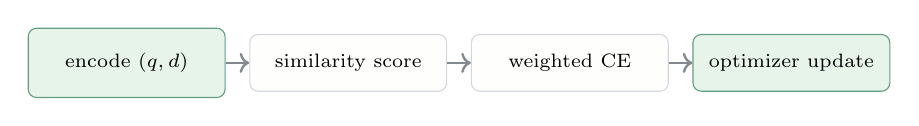
\begin{tikzpicture}[node distance=0.28cm and 0.30cm]
        \node[flowgreen,minimum width=2.50cm,minimum height=0.88cm,font=\scriptsize] (enc) {encode $(q,d)$};
        \node[flow,minimum width=2.50cm,font=\scriptsize] (score) [right=of enc] {similarity score};
        \node[flow,minimum width=2.50cm,font=\scriptsize] (loss) [right=of score] {weighted CE};
        \node[flowgreen,minimum width=2.50cm,font=\scriptsize] (update) [right=of loss] {optimizer update};
        \draw[arrow] (enc) -- (score);
        \draw[arrow] (score) -- (loss);
        \draw[arrow] (loss) -- (update);
    \end{tikzpicture}

    \begin{center}
        \keynote{两张 A40 各处理 1 个 candidate group，gather 后另一 query 的候选文档作为 in-batch negatives\\我们先计算每个 query 的对比交叉熵，随后按对应 Training pair 的 \texttt{reweight\_rate} 加权。}
    \end{center}
    \begin{columns}[T,onlytextwidth]
        \column{0.46\textwidth}
        \sectionhead{目标函数}
        \colorbox{softBlue}{\parbox{0.94\linewidth}{\centering
            $\displaystyle s(q,d)=\frac{q^{\top}d}{\tau},\quad \tau=0.02$\\[0.5mm]
            $\displaystyle \mathcal{L}=\frac{\sum_j w_j\ell_j}{\sum_j w_j}$\\
            {\footnotesize\textcolor{mutedGray}{$\ell_j$：query $j$ 对比交叉熵；\\ $w_j$：Training pair 的 \texttt{reweight\_rate}。}\\
            \textcolor{mutedGray}{权重在每个 2-query micro-batch 内归一化。}}}}
        \column{0.46\textwidth}
        \sectionhead{批次组织}
        \footnotesize
        \begin{tabular}{@{}ll@{}}
            硬件 & 2 $\times$ A40\\
            micro-batch & 2 groups\\
            梯度累积 & 4 micro-steps\\
            optimizer update & per 8 candidate groups\\
        \end{tabular}
    \end{columns}
\end{frame}

\begin{frame}{3.5 训练配置选择：先确定训练轮数，再选择学习率}
    \begin{columns}[T,onlytextwidth]
        \column{0.47\textwidth}
        \sectionhead{训练轮数}
        {\centering\small 我们固定 LR=$10^{-6}$，使用完整 96,504 条 \\ Training pairs，分别训练 1、2、3 epoch \\ 并提交模型至 A 榜，结果如下：\par}
        {\centering\scriptsize
        \begin{tabular}{lrrrr}
            \toprule
                epoch & Total & Recall & Success & Avg\_Steps \\
                \midrule
                \rowcolor{softBlue}\textbf{1} & \textbf{40.1} & 44.8 & 21.0 & 15.4 \\
                2 & 38.2 & 42.7 & 18.3 & 15.5 \\
                3 & 38.7 & 43.4 & 19.0 & 15.8 \\
            \bottomrule
        \end{tabular}
        \par}
        \smallnote{完整 pairs 上的实验确定使用 1 epoch；随后在 query-disjoint 训练阶段选择学习率。}

        \column{0.43\textwidth}
        \sectionhead{学习率（LR）}
        {\centering\small 固定 query-disjoint train（94,113 rows），\\ 四个 LR 各训练 500 个 optimizer steps，\\ 随后在 dev1500 上比较 R@1 与 MRR：\par}
        {\centering\scriptsize
        \begin{tabular}{lrr}
            \toprule
            学习率 & R@1 & MRR \\
            \midrule
            $3\times10^{-7}$ & 0.4913 & 0.6419 \\
            $5\times10^{-7}$ & 0.5073 & 0.6571 \\
            $1\times10^{-6}$ & 0.5433 & 0.6831 \\
            \rowcolor{softBlue}\textbf{$2\times10^{-6}$} & \textbf{0.5640} & \textbf{0.6993} \\
            \bottomrule
        \end{tabular}\par}
        \smallnote{R@1 和 MRR 同时在 LR=$2\times10^{-6}$ 时最高，因此选择该学习率。}\par
    \end{columns}
    \begin{center}
        \keynote{最终采用：1 epoch + LR=$2\times10^{-6}$。}
    \end{center}
\end{frame}

\begin{frame}{4.1 A 榜结果：整体方案与内部学习率对照}
    \centering
    {\scriptsize
    \begin{tabular}{@{}p{6.00cm}rrrr@{}}
        \toprule
        配置 & Total $\uparrow$ & Recall $\uparrow$ & Success $\uparrow$ & Avg\_Steps $\downarrow$ \\
        \midrule
        Baseline Qwen3 Embedding & 28.5 & 28.5 & 10.6 & 17.8 \\
        Baseline LRAT: 2 epochs, LR = 1e-6 & 34.0 & 36.1 & 15.5 & 16.8 \\
        Query-disjoint: 1 epochs, LR = 1e-6 & 39.5 & 45.0 & 19.8 & 15.9 \\
        \rowcolor{softBlue}\textbf{Query-disjoint: 1 epochs, LR = 2e-6} & \textbf{40.6} & \textbf{46.3} & \textbf{21.1} & \textbf{16.0} \\
        \bottomrule
    \end{tabular}
    }

    \footnotesize\textcolor{mutedGray}{\textbf{Total}：综合得分；\textbf{Recall}：检索器召回率；\textbf{Success}：端到端成功率；\textbf{Avg\_Steps}：平均执行轮次。}\\

    \vspace{1mm}
    \begin{columns}[T,onlytextwidth]
        \column{0.48\textwidth}
        \sectionhead{平台结果}
        \small
        Baseline Qwen3：28.5 $\rightarrow$ 40.6（$+12.1$）。\\
        Baseline LRAT：34.0 $\rightarrow$ 40.6（$+6.6$）。
        \column{0.48\textwidth}
        \sectionhead{内部学习率调整}
        \small 在同一 query-disjoint 设置下，将 LR 从 $10^{-6}$ 调至 $2\times10^{-6}$，Total 从 39.5 提升至 40.6。
    \end{columns}
\end{frame}

\begin{frame}{4.2 B 榜结果：复现验收与三种 Agent 的实测结果}
    \centering
    \begin{tikzpicture}[node distance=0.25cm and 0.42cm]
        \node[flow,minimum width=2.70cm,font=\scriptsize] (ckpt) {final retriever};
        \node[flowgreen,minimum width=2.70cm,font=\scriptsize] (freeze) [right=of ckpt] {冻结并记录模型身份};
        \node[flow,minimum width=2.70cm,font=\scriptsize,align=center] (agent) [right=of freeze] {接入三个 Agent\\进行 B 榜实测};
        \draw[arrow] (ckpt) -- (freeze);
        \draw[arrow] (freeze) -- (agent);
    \end{tikzpicture}

    \begin{columns}[T,onlytextwidth]
        \column{0.45\textwidth}
        \sectionhead{复现验收}
        \footnotesize
        \begin{tabular}{@{}>{\raggedright\arraybackslash}p{0.98\linewidth}@{}}
            \textcolor{accentRed}{\tiny$\bullet$}\hspace{0.4em}固定模型、代码和关键配置的身份；\\[1.2mm]
            \textcolor{accentRed}{\tiny$\bullet$}\hspace{0.4em}用新 CPU 进程独立加载最终模型；\\[1.2mm]
            \textcolor{accentRed}{\tiny$\bullet$}\hspace{0.4em}回读 Hugging Face revision 并核对文件哈希；\\[1.2mm]
            \textcolor{accentRed}{\tiny$\bullet$}\hspace{0.4em}GitHub repository 与本地文件校验。
        \end{tabular}
        \column{0.45\textwidth}
        \sectionhead{B 榜结果}
        \footnotesize
        \begin{tabular}{@{}>{\raggedright\arraybackslash}p{0.98\linewidth}@{}}
            \textcolor{accentRed}{\tiny$\bullet$}\hspace{0.4em}DeepSeek-V4-Flash-0731：Total 67.42；\\[1.2mm]
            \textcolor{accentRed}{\tiny$\bullet$}\hspace{0.4em}Qwen3.5-35B-A3B：Total 60.96；\\[1.2mm]
            \textcolor{accentRed}{\tiny$\bullet$}\hspace{0.4em}gpt-oss-120b：Total 40.16；\\[1.2mm]
            \textcolor{accentRed}{\tiny$\bullet$}\hspace{0.4em}平均 Total 56.18，最高与最低相差 27.26。
        \end{tabular}
        \vspace{1.5mm}
        \smallnote{\parbox{0.98\linewidth}{注：未提供逐 Agent baseline，因此本页只报告三种 Agent 的绝对表现，不作相对提升判断。}}
    \end{columns}
\end{frame}

\newcommand{\factcard}[5]{%
    \node[#1,text width=4.25cm,minimum height=3.40cm,align=left] at (#2,0) {%
        \begin{minipage}[t][4.00cm][t]{3.82cm}
            \centering
            {\textcolor{accentRed}{\Large\bfseries #3}}\\[1.5mm]
            {\textcolor{navyBlue}{\bfseries #4}}\\[2mm]
            #5
        \end{minipage}%
    };
}

\begin{frame}{5. 总结：我们做了什么，结果说明什么}
    \centering
    \begin{tikzpicture}
        \factcard{card}{-5.00cm}{01}{数据链路}{%
            \begin{tabular}{@{}>{\raggedright\arraybackslash}p{3.82cm}@{}}
                \scriptsize\textcolor{accentRed}{\tiny$\bullet$}\hspace{0.4em}从 Training pairs 追溯核验到 trajectory / Corpus\\[0.6mm]
                \scriptsize\textcolor{accentRed}{\tiny$\bullet$}\hspace{0.4em}normalized query 按 group 完成整组隔离
            \end{tabular}}
        \factcard{card}{0cm}{02}{结果}{%
            \begin{tabular}{@{}>{\raggedright\arraybackslash}p{3.82cm}@{}}
                \scriptsize\textcolor{accentRed}{\tiny$\bullet$}\hspace{0.4em}A 榜最终 Total 为 40.6\\[0.6mm]
                \scriptsize\textcolor{accentRed}{\tiny$\bullet$}\hspace{0.4em}相比 Baseline LRAT 34.0，提高 6.6\\[0.6mm]
                \scriptsize\textcolor{accentRed}{\tiny$\bullet$}\hspace{0.4em}B 榜三 Agent 平均：56.18
            \end{tabular}}
        \factcard{accentcard}{5.00cm}{03}{关键发现}{%
            \begin{tabular}{@{}>{\raggedright\arraybackslash}p{3.82cm}@{}}
                \scriptsize\textcolor{accentRed}{\tiny$\bullet$}\hspace{0.4em}同一 query-disjoint 设置调整 LR：39.5 $\rightarrow$ 40.6\\[0.6mm]
                \scriptsize\textcolor{accentRed}{\tiny$\bullet$}\hspace{0.4em}三个 Agent Total 相差 27.26，同一 retriever 的绝对表现对具体 Agent 仍然敏感
            \end{tabular}}
    \end{tikzpicture}
\end{frame}

\end{document}
